\documentclass[tikz,border=8pt]{standalone}
\usepackage{amsmath,amssymb}
\usetikzlibrary{arrows.meta,automata,positioning,quotes}
\begin{document}
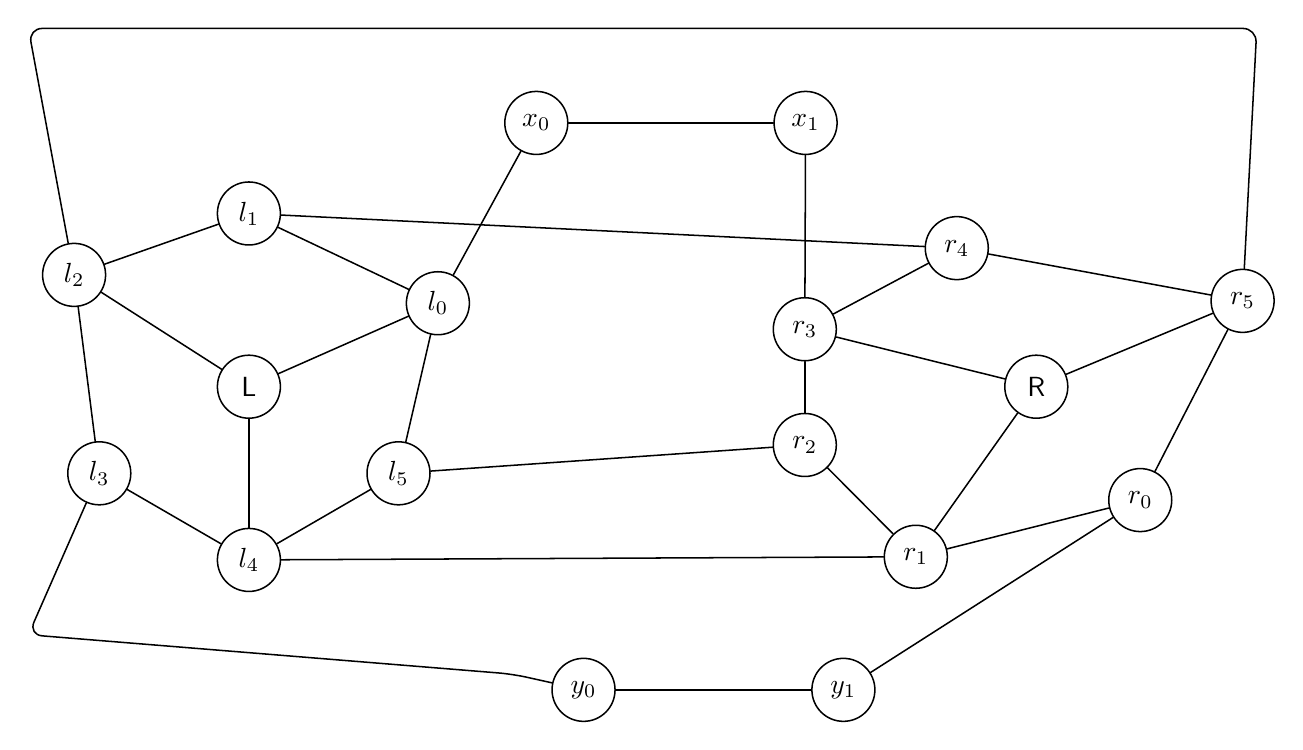
\begin{tikzpicture}[x=1cm,y=1cm]
\tikzset{
  graphnode/.style={circle,draw=black,line width=0.55pt,minimum size=8mm,inner sep=1pt,font=\sffamily},
  graphedge/.style={draw=black,line width=0.55pt,line cap=round,line join=round},
  directed/.style={graphedge,-{Stealth[length=2.4mm,width=2.0mm]}},
  undirected/.style={graphedge}
}
\node[graphnode] (n_L) at (-5.00,0.00) {L};
\node[graphnode] (n_l0) at (-2.60,1.06) {$l_{0}$};
\node[graphnode] (n_l1) at (-5.00,2.20) {$l_{1}$};
\node[graphnode] (n_l2) at (-7.22,1.42) {$l_{2}$};
\node[graphnode] (n_l3) at (-6.90,-1.10) {$l_{3}$};
\node[graphnode] (n_l4) at (-5.00,-2.20) {$l_{4}$};
\node[graphnode] (n_l5) at (-3.10,-1.10) {$l_{5}$};
\node[graphnode] (n_R) at (5.00,0.00) {R};
\node[graphnode] (n_r0) at (6.32,-1.44) {$r_{0}$};
\node[graphnode] (n_r1) at (3.47,-2.16) {$r_{1}$};
\node[graphnode] (n_r2) at (2.06,-0.74) {$r_{2}$};
\node[graphnode] (n_r3) at (2.06,0.73) {$r_{3}$};
\node[graphnode] (n_r4) at (3.99,1.76) {$r_{4}$};
\node[graphnode] (n_r5) at (7.62,1.09) {$r_{5}$};
\node[graphnode] (n_x0) at (-1.35,3.35) {$x_{0}$};
\node[graphnode] (n_x1) at (2.07,3.35) {$x_{1}$};
\node[graphnode] (n_y0) at (-0.75,-3.85) {$y_{0}$};
\node[graphnode] (n_y1) at (2.55,-3.85) {$y_{1}$};
\draw[undirected] (n_l0) -- (n_l1);
\draw[undirected] (n_l1) -- (n_l2);
\draw[undirected] (n_l2) -- (n_l3);
\draw[undirected] (n_l3) -- (n_l4);
\draw[undirected] (n_l4) -- (n_l5);
\draw[undirected] (n_l5) -- (n_l0);
\draw[undirected] (n_L) -- (n_l0);
\draw[undirected] (n_L) -- (n_l2);
\draw[undirected] (n_L) -- (n_l4);
\draw[undirected] (n_r0) -- (n_r1);
\draw[undirected] (n_r1) -- (n_r2);
\draw[undirected] (n_r2) -- (n_r3);
\draw[undirected] (n_r3) -- (n_r4);
\draw[undirected] (n_r4) -- (n_r5);
\draw[undirected] (n_r5) -- (n_r0);
\draw[undirected] (n_R) -- (n_r1);
\draw[undirected] (n_R) -- (n_r3);
\draw[undirected] (n_R) -- (n_r5);
\draw[undirected] (n_l0) -- (n_x0);
\draw[undirected] (n_x0) -- (n_x1);
\draw[undirected] (n_x1) -- (n_r3);
\draw[undirected,rounded corners=5pt] (n_l3) -- (-7.80,-3.15) -- (-1.65,-3.65) -- (n_y0);
\draw[undirected] (n_y0) -- (n_y1);
\draw[undirected] (n_y1) -- (n_r0);
\draw[undirected] (n_l1) -- (n_r4);
\draw[undirected,rounded corners=5pt] (n_l2) -- (-7.80,4.55) -- (7.80,4.55) -- (n_r5);
\draw[undirected] (n_l4) -- (n_r1);
\draw[undirected] (n_l5) -- (n_r2);
\end{tikzpicture}
\end{document}
